%!TEX root = ./template-skripsi.tex

\subsection{\textit{Sprint 4}}

	\textit{Sprint-4} dilakukan sepekan pada tanggal 13 September 2022 sampai dengan 20 september 2022. \textit{Story} keempat pada \textit{product backlog} yaitu membuat grading berat dipecah menjadi beberapa \textit{task} sebagai berikut.


 \begin{longtable}[c]{@{} |p{1cm}|p{4cm}|p{5cm}|p{3cm}| @{}}
 \caption{\textit{Sprint 4} \label{sprint4_table}}\\


 \hline
  \multirow{1}{=}{\centering{\textbf{No}}} & \multirow{1}{=}{\centering{\textbf{\textit{Story}}}} & \multirow{1}{=}{\centering{\textbf{\textit{Task}}}} & \multirow{1}{=}{\centering{\textbf{\textit{Status}}}}\\
 \endfirsthead

 \hline
  \multirow{1}{=}{\centering{\textbf{No}}} & \multirow{1}{=}{\centering{\textbf{\textit{Story}}}} & \multirow{1}{=}{\centering{\textbf{\textit{Task}}}} & \multirow{1}{=}{\centering{\textbf{\textit{Status}}}}\\
 \endhead

 \hline
 \endfoot

 \hline
 \endlastfoot

 \hline
 1 & Membuat fitur grading berat ikan &  Membuat \textit{Mock-up UI} halaman rekapitulasi grading, detail grading, entry grading  &  selesai \\
 \hline
 2 & & Menerapkan \textit{Mock-up UI} halaman rekapitulasi grading, detail grading, entry grading ke Flutter & selesai\\
 \hline
 3 & & Mengintegrasikan halaman rekapitulasi grading, detail grading, entry grading ke \textit{webservice} & selesai\\
 \hline
 \end{longtable}

Pada sprint keempat ini story yang di pilih untuk di uraikan pada sprint kali ini adalah membuat halaman rekapitulasi grading, detail grading, entry grading. Tujuan dari \textit{sprint-4} ini adalah membuat fitur grading berat ikan dan mengintegrasikan halaman tersebut dengan webservice yang sudah dibuat oleh penelitian Andri Rahmanto.

\begin{enumerate}[listparindent=2em]
	
	\item{\textit{Membuat Mock-up UI Fitur Grading}}
	
	Pembuatan konten dan fitur yang terdapat pada \textit{mock-up UI} fitur grading dilakukan berdasarkan persetujuan product owner dan scrum master pada meeting sebelumnya. Mock-up UI dibuat menggunakan platform figma.
	
	\begin{figure}[H]
	\centering
	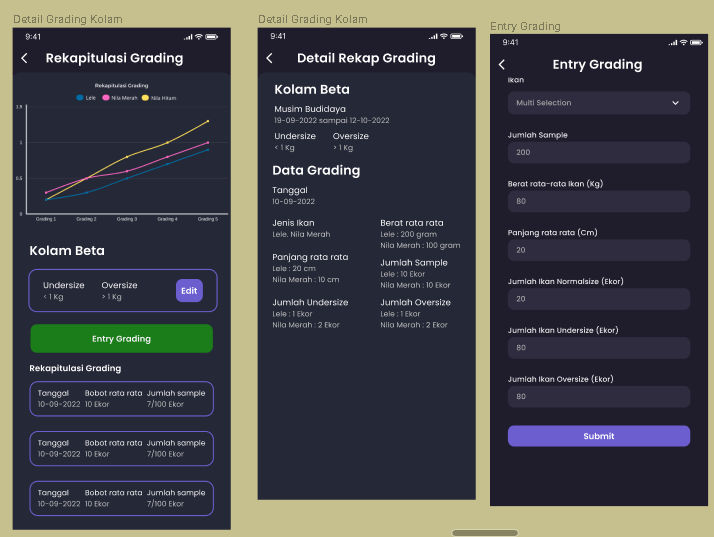
\includegraphics[keepaspectratio, width=6cm]{gambar/mockupgrading}
	\caption{\textit{Mock-up UI Fitur Grading}}
	\label{gambar:mockupgrading}
	\end{figure}

	\item{\textit{Class Diagram}}
	
	Class Diagram menggambarkan kelas-kelas yang akan dipakai oleh sistem. Umumnya terdapat 3 kelas pada setiap module yaitu class model, controller, dan view. Pada sprint-4 penelitian kali ini penulis membuat 4 class yaitu model yang berwarna biru, view berwarna oranye, controller yang berwarna hijau, dan service yang berwarna kuning.
	 
	 \begin{figure}[H]
	 \centering
	 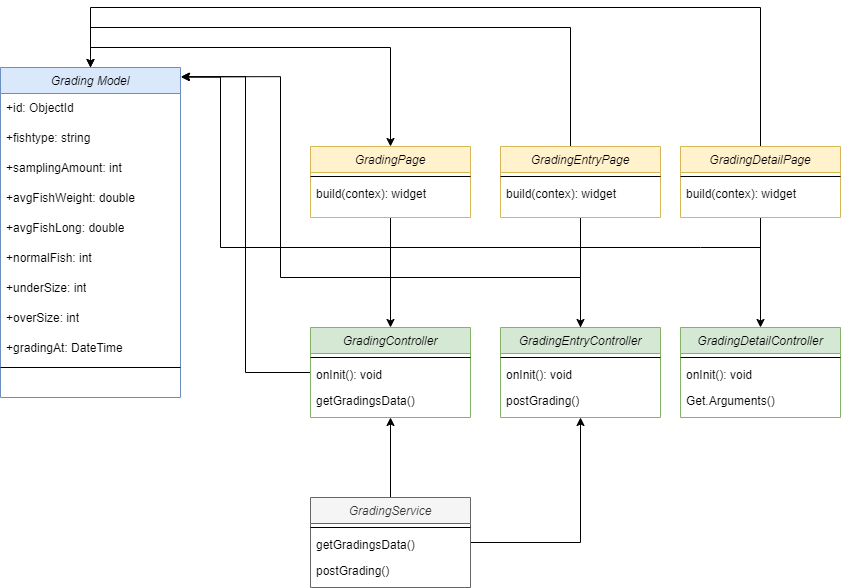
\includegraphics[keepaspectratio, width=6cm]{gambar/gradingcd}
	 \caption{\textit{Class Diagram Fitur Sprint-4}}
	 \label{gambar:gradingcd}
	 \end{figure}


	\item{\textit{Menerapkan Mockup-UI Fitur Grading kedalam code flutter}}
	
	Setelah \textit{mock-up UI fitur grading} hingga prototype dibuat, akan dilakukan pengimplementasian \textit{mock-up UI} ke dalam aplikasi menggukan flutter. Source code dari implementasi fitur grading terdapat pada lampiran 5 yang menghasilkan output halaman sebagai berikut
	
	\begin{figure}[H]
		\centering
		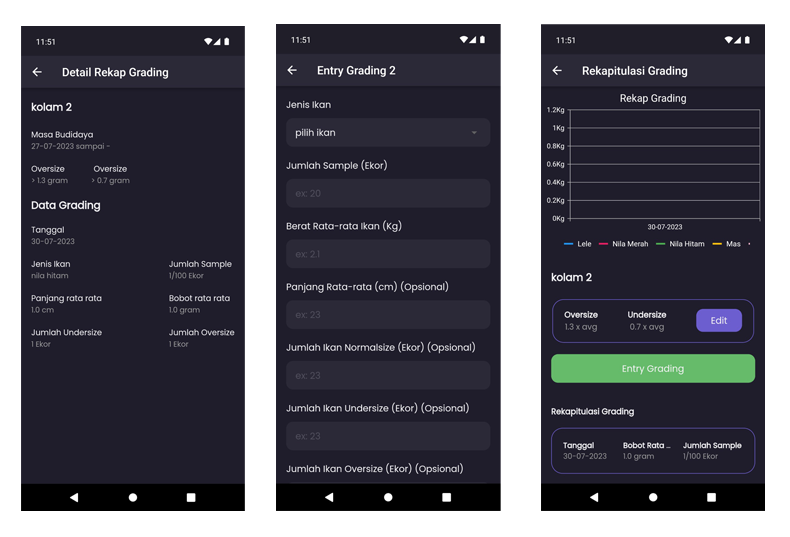
\includegraphics[keepaspectratio, width=8cm]{gambar/sssprint4}
		\caption{\textit{Output dari code pada sprint 4}}
		\label{gambar:sssprint4}
		\end{figure}

	\item{\textit{Mengitegrasikan fitur grading dengan webservice}}

	Sebelumnya, setiap data pada fitur masih berupa data dummy sehingga perlu diintegrasikan dengan webservice agar aplikasi dapat berjalan dengan data yang asli. Hal yang dilakukan dalam mengintegrasikan fitur grading dengan webservice terdapat pada lampiran 5.
	
  \item{Analisis \textit{User Experience}} 
 
  Pada halaman grading, pembudidaya harus jenis ikan dan data klasifikasi ukuran ikan. Di halaman rekapitulasi grading, terdapat grafik mengenai statistik pertumbuhan ikan  pada musim budidaya yang berjalan sehingga pembudidaya dapat dengan mudah mengetahui perkembangan ukuran ikan dari waktu ke waktu, selain itu terdapat juga list mengenai grading yang telah dilakukan yang berisi informasi yang berhubungan dengan ukuran ikan saat dilakukan grading.

\item{Sprint 4 Review dan Sprint 5 Planning}

Sprint 4 diakhiri dengan melakukan weekly meeting pada hari selasa dengan agenda melakukan review dan testing terkait hasil sprint 4 dan melakukan planning untuk sprint 5 dengan rincian:
\begin{enumerate}
	\item{\textit{Review dan Testing hasil dari sprint 4}}

	Telah dilakukan review dan testing oleh penulis selaku developer dengan Scrum Master. Setelah dilakukan testing, Scrum Master menyimpulkan bahwa fitur grading berat ikan telah berjalan dengan baik.
\begin{longtable}{| p{8cm} | c | c | l |}
  \caption{Unit testing Halaman Rekapitulasi Grading.\label{table:unit_testing_rekapitulasi_grading}}\\
  \hline
  \multirow{2}{*}{Skenario Pengujian} & \multicolumn{2}{l|}{Kesesuaian} & \multirow{2}{*}{Kesimpulan} \\ 
  \cline{2-3}
    & \multicolumn{1}{l|}{sesuai} & tidak sesuai & \\ 
  \hline
  \hline
  \endfirsthead
  \hline
  \multirow{2}{*}{Skenario Pengujian} & \multicolumn{2}{l|}{Kesesuaian} & \multirow{2}{*}{Kesimpulan} \\ 
  \cline{2-3}
    & \multicolumn{1}{l|}{sesuai} & tidak sesuai &  \\ 
  \hline
  \hline
  \endhead
  \hline
  \endfoot
  
  
  \hline\hline
  \endlastfoot
  Ketika menekan list data rekapitulasi grading, maka akan ditamplikan detail rekapitulasi grading & \Checkmark &  & Diterima \\ 
  \hline
  Ketika menekan list data rekapitulasi grading, maka akan ditamplikan detail rekapitulasi grading & \Checkmark &  & Diterima \\ 
  \hline
  Saat tombol entry grading ditekan maka akan menampilkan halaman entry grading & \Checkmark &  & Diterima \\ 
  \hline
  ketika mengisi form rekapitulasi grading dengan data yang sesuai dan menekan submit, data rekapitulasi grading akan ditambahkan & \Checkmark &  & Diterima \\ 
  \hline
  \end{longtable}

	\item{\textit{Sprint Planning untuk Sprint 5}}
	
	Planning untuk sprint 5 yakni membuat fitur rekapitulasi kematian ikan pada aplikasi \textit{Assistive Aquaculture Breeding Management}.
\end{enumerate}
\end{enumerate}	